\documentclass[12pt]{article}
\usepackage{scrextend}
\usepackage[utf8]{inputenc}
\usepackage[polish]{babel}
\usepackage[T1]{fontenc}%polskie znaki
\usepackage[utf8]{inputenc}%polskie znaki
\usepackage{geometry}
\usepackage{float}
\usepackage{enumitem}
\usepackage{hyperref}
\usepackage{graphicx}
\usepackage{tabulary}
\usepackage{etoc}
\usepackage[normalem]{ulem} 
\usepackage{tikz}
\usepackage[bf]{caption}
\usepackage{amsmath}

\renewcommand{\baselinestretch}{1.5}

\usepackage{listings}
\usepackage{xcolor}
 
\definecolor{codegreen}{rgb}{0,0.6,0}
\definecolor{codegray}{rgb}{0.5,0.5,0.5}
\definecolor{codepurple}{rgb}{0.58,0,0.82}
\definecolor{backcolour}{rgb}{0.95,0.95,0.92}
 
\lstdefinestyle{mystyle}{
    backgroundcolor=\color{backcolour},   
    commentstyle=\color{codegreen},
    keywordstyle=\color{magenta},
    numberstyle=\tiny\color{codegray},
    stringstyle=\color{codepurple},
    basicstyle=\ttfamily\footnotesize,
    breakatwhitespace=false,         
    breaklines=true,                 
    captionpos=b,                    
    keepspaces=true,                 
    numbers=left,                    
    numbersep=5pt,                  
    showspaces=false,                
    showstringspaces=false,
    showtabs=false,                  
    tabsize=2
}
\renewcommand{\lstlistlistingname}{Spis listingów}\lstset{style=mystyle}

\graphicspath{ {img/} }
\newgeometry{lmargin=2.0cm, rmargin=2.0cm, tmargin=2.0cm, bmargin=2.0cm}
\clubpenalty=9996
\widowpenalty=9999
\brokenpenalty=4991
\predisplaypenalty=10000
\postdisplaypenalty=1549
\displaywidowpenalty=1602

\title{ 
    \vspace*{50mm}
    \textsc{
        \textbf{Grafika komputerowa}\\
        \large Sprawozdanie 
    }
} 
\author{
Damian Koper,  241292\\
}

\date{\today}

\begin{document}

\maketitle

\newpage
\setcounter{tocdepth}{2}
\localtableofcontents
\listoffigures
\lstlistoflistings

\newpage


\section{OpenGL - podstawy}

OpenGL (\textit{Open Graphics Library}) stanowi otwarty i~uniwersalny interfejs umożliwiający renderowanie grafiki 2D i~3D. Obliczenia realizowane są dzięki bezpośredniej interakcji z~GPU, który, mając zaimplementowane potrzebne operacje, może szybko przeprowadzać obliczenia. Natura abstrakcyjnego interfejsu jakim jest OpenGL pozwala tworzyć przenośne programy renderujace grafikę bez zważania na platformę uruchomienia, gdzie obliczenia mogą być realizowane programowo jak i~sprzętowo.

\subsection{Bazowa aplikacja}
Biblioteką, która tworzy środowisko uruchomieniowe dla wyświetlania wyrenderowanej grafiki i~realizuje operacje wejścia-wyjścia jest GLUT (\textit{OpenGL Utility Toolkit}). Prosty program wyświetlajacy okno można stworzyć niewielkim nakładem pracy.

\begin{lstlisting}[language=C++, caption=Bazowy program wyświetlający czarne okno.]
#include <GL/glut.h>
void draw()
{
  glClearColor(0, 0, 0, 1);
  glClear(GL_COLOR_BUFFER_BIT);
  glFlush();
}

int main(int argc, char **argv)
{
  glutInit(&argc, argv);
  glutInitDisplayMode(GLUT_SINGLE | GLUT_RGB);
  glutInitWindowPosition(50, 50);
  glutInitWindowSize(800, 800);
  glutCreateWindow("Lab GK");
  glutDisplayFunc(draw);
  glutMainLoop();
  return 0;
}
\end{lstlisting}

W funkcji \lstinline{main} w pierwszej kolejności inicjalizowana jest sama aplikacja, a następnie wszystkie jej parametry. Następnie do biblioteki GLUT przekazywana poprzez wskaźnik jest funkcja \lstinline{draw}, ktora jest odpowedzialna za bezpośrednią interakcję z API OpenGL, a zatem za rysowanie właściwych elementów w wyświetlonym oknie. W tej wersji funkcja \lstinline{draw} czyści okno kolorem czarnym i opróżnia bufor przekazując dane na ekran.

\subsection{Dywan Sierpińskiego}
Dywan Sierpińskiego jest jest fraktalem otrzymanym z kwadratu podzielonego na 9 mniejszych kwadratów, z których usuwany jest środkowy. Procedura ta jest rekurencyjnie powtarzana dla pozostałych ośmiu kwadratów.
\begin{figure}[h]
  \centering
  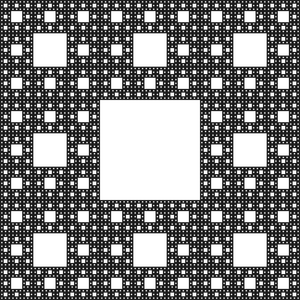
\includegraphics[width=0.3\linewidth]{img/300px-Sierpinski6.png}
  \caption{Dywan Sierpińskiego po 6 iteracjach.}
\end{figure}

\subsubsection{Rysowanie rekurencyjne}
Rysowanie dywanu Sierpińskiego zrealizowane za pomocą rekurencji zakłada rekurencyjne wywołanie funkcji dla każdego z ośmiu zewnętrznych kwadratów fraktalu. Poziomów wywoływań następuje tyle ile zostało zdefiniowane dla pierwszego wywołania funkcji. Gdy zostanie spełniony warunek zakończenia rekurencji, rysowany jest kwadrat. Funkcja po raz pierwszy zostaje wywołana w metodzie \lstinline{draw} zaraz po wyczyszczeniu okna.

\begin{figure}[H]
  \
  \begin{minipage}[t]{.45\linewidth}
      
\includegraphics[width=\linewidth]{img/serpinski_3_s1.png}
      \caption{Częściowo narysowany dywan Sierpińskiego po zakończeniu 30 gałęzi rekurencji.}
  \end{minipage}
  \hspace{.05\linewidth}
  \begin{minipage}[t]{0.45\linewidth}
      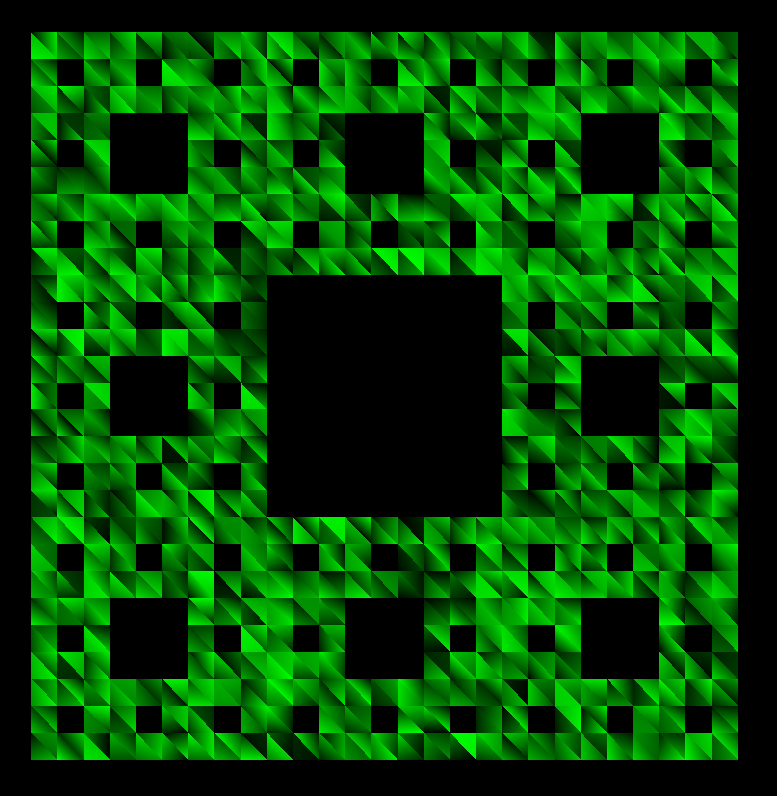
\includegraphics[width=\linewidth]{serpinski_3_s2}
      \caption{Dywan Sierpińskiego narysowany w całości.}
  \end{minipage}
\end{figure}

\begin{lstlisting}[language=C++, caption=Funkcja rysująca dywan Sierpińskiego rekurencyjnie. Pominięto niektóre wywołania.]
void carpet(int levels, float a, float dx = 0, float dy = 0)
{
  if (levels != 0)
  {
    a = a / 3;
    carpet(levels - 1, a, dx - a, dy - a);
    ...
    carpet(levels - 1, a, dx + a, dy + a);
  }
  else
  {
    //Pomocnicza funkcja rysujaca kwadrat
    rect(dx, dy, a); 
  }
}
\end{lstlisting}
\subsubsection{Rysowanie iteracyjne}
Rysowanie iteracyjne możliwe jest do osiągnięcia przez matematyczne sprawdzenie czy dany kwadrat ma być wypełniony czy nie, albo zamianę wersji rekurencyjnej do wersji iteracyjnej z wykorzystaniem kolejki i struktury danych opisującej aktualny poziom rysowania.

\begin{lstlisting}[language=C++, caption=Struktura danych przechowująca aktualny stan rysowania.]
struct CarpetLevelData
{
  int level;
  float a;
  float dx = 0;
  float dy = 0;
};
\end{lstlisting}


\begin{lstlisting}[language=C++, caption=Funkcja rysująca dywan Sierpińskiego iteracyjnie. Pominięto niektóre wywołania.]
void carpetIt(int levels, float a)
{
  queue<CarpetLevelData> q = queue<CarpetLevelData>();
  q.push({levels, a});
  while (!q.empty())
  {
    CarpetLevelData data = q.front();
    if (data.level > 0)
    {
      data.a = data.a / 3;
      q.push({data.level - 1, data.a, data.dx - data.a, data.dy - data.a});
      ...
      q.push({data.level - 1, data.a, data.dx + data.a, data.dy + data.a});
    }
    else
    {
      rect(data.dx, data.dy, data.a);
    }
    q.pop();
  }
\end{lstlisting}

\subsubsection{Losowe kolory i perturbacje}
Losowe kolory osiągnięto poprzez wywołanie funkcji \lstinline{glColor3ub(0, randChar(), 0)} przed wywołaniem funkcji interfejsu OpenGL definiującą składowy wierzchołek trojąta tworzącego kwadrat, gdzie funkcja \lstinline{randChar} zwraca liczbę z przedziału $<0;255>$. Mając kontrolę nad rysowanem każdego kwadratu można wprowadzić również losowe jego przesunięcie w osi X i Y.

\begin{figure}[h]
  \centering
  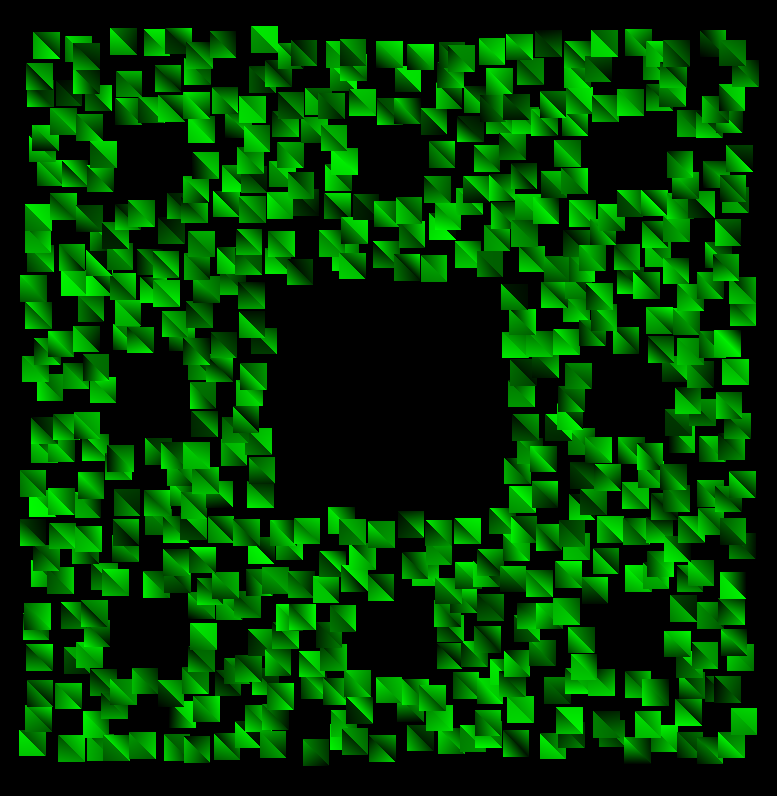
\includegraphics[width=0.4\linewidth]{img/serpinski_3_s3.png}
  \caption{Dywan Sierpińskiego po 3 iteracjach z losowym kolorem zielonym oraz perturbacjami.}
\end{figure}
\newpage
\section{Modelowanie obiektów 3D}
\subsection{Bazowa aplikacja}
Aplikacja bazowa, po zainicjowaniu niezbędnych elementów biblioteki \textit{GLUT}, oddaje sterowanie do utworzonej klasy \lstinline{ViewEngine}. Przechowuje one referencje na klasy, będące niezależnymi widokami. Widoki te posiadają zdefiniowane własne funkcje odpowiedzialne za renderowanie, obsługę zdarzeń, animację oraz obsługę zdarzeń związanych z~cyklem życia widoku. Poprzez zmianę wartości wskaźnika na aktualny widok w klasie \lstinline{ViewEngine}, funkcje przekazane do biblioteki \textit{GLUT} zastępowane są funkcjami właściwego widoku. Każdy widok musi implementować interfejs \lstinline{iView} zdefiniowany następująco:

\begin{lstlisting}[language=C++, caption=Interfejs IView.]
class IView
{
public:
    virtual std::string getName() = 0;
    virtual void init() = 0;
    virtual void onEnter() = 0;
    virtual void render() = 0;
    virtual void idle() = 0;
    virtual void timer() = 0;
    virtual void onKey(unsigned char key, int x, int y) = 0;
    virtual void onLeave() = 0;

    virtual ~IView(){};
};
\end{lstlisting}
Widoku identyfikowane są za pomocą nazw zwracanych przez funkcję \lstinline{getName()}.
Dzięki zaimplementowaniu wzorca Singleton w klasie \lstinline{ViewEngine} możliwe jest przełączanie widoku w dowolnym miejscu wywołania metody w programie.
\begin{lstlisting}[language=C++, caption=Tworzeznie instancji widoków i~ustawianie obecnego. Funkcja \lstinline{g} zwraca instancję klasy.]
ViewEngine::g().add(new TeapotView());
ViewEngine::g().add(/*inne widoki*/);
ViewEngine::g().setCurrent("complexEgg");
\end{lstlisting}
\subsection{Model i~generowanie punktów}
\subsubsection{Generowanie punktów}
W ćwiczeniu wygenerowane zostały punkty modelu jajka. Uzyskane zostały poprzez obrócenie odpowiednio dobranej krzywej Beziera. Punkty opisują wzory w dziedzinie parametrycznej kwadratu jednostkowego:
\begin{align*}
    x(u,v)&=(-90u^5+225u^4-270u^3+180u^2-45u)cos(\pi v)\\
    y(u,v)&=160u^4-320u^3+160u^2\\
    z(u,v)&=(-90u^5+225u^4-270u^3+180u^2-45u)sin(\pi v)
\end{align*}
Generowanie punktów dla wartości parametrów funkcji z~przedziału $<0;1>$ zakłada wygenerowanie nakładających się punktów. Dlatego w programie pominięto ostatnie iteracje pętli.
\subsubsection{Model}
Każdy model zdefiniowany jest za pomocą klasy, która przyjmuje parametry określające jego wygląd i~zachowania. W przypadku klasy \lstinline{Egg} jest to ilość iteracji pętli generowania punktów, co przekłada się na poziom wygładzenia modelu. Klasa modelu odpowiedzialna jest również za jego rysowanie w różnych wariantach.

Dla czytelności kodu stworzona została klasa \lstinline{Point}, która przechowuje współrzędne punktu, jego kolor, oraz odpowiedzialna jest rysowanie samego siebie.

\begin{lstlisting}[language=C++, caption=Nagłówek klasy Point.]
class Point
{
public:
    Point(float x, float y, float z, GLubyte r, GLubyte g, GLubyte b)
        : color({r, g, b}), x(x), y(y), z(z){};
    ~Point();
    void callGlVertex3f();
    void callGlColor3f();
    void drawWithColor();
    struct Color
    {
        GLubyte r = 255;
        GLubyte g = 255;
        GLubyte b = 255;
    };
    float x = 0;
    float y = 0;
    float z~= 0;
    Color color;
};
\end{lstlisting}
Właściwa generacja punktów odbywa się w konstruktorze klasy \lstinline{Egg}.
\begin{lstlisting}[language=C++, caption=Nagłówek klasy modelu Egg.]
class Egg
{
public:
    Egg(int n = 32);
    ~Egg();
    std::vector<std::vector<Point>> getPoints();
    void renderPoints();
    void renderMesh();
    void renderTriangles();
    void renderComplex();
private:
    int n;
    std::vector<std::vector<Point>> points;
    float calcX(float u, float v);
    float calcY(float u, float v);
    float calcZ(float u, float v);
};
\end{lstlisting}
\newpage
\subsection{Rysowanie modelu za pomocą punktów, siatki i~jako bryły}

W utworzonej aplikacji rysowanie odbywa się w metodzie \lstinline{IView::render()} modelu. Znajduje się tam również opisana niżej procedura transformacji i~animacji modelu.
\subsubsection{Rysowanie punktów}
Rysowanie punktów obywa się z~wykorzystanie prymitywu \lstinline{GL_POINTS} biblioteki \textit{OpenGL}. Wszystkie punkty podawane są do funkcji w dowolnej kolejności.

\begin{lstlisting}[label={lst:anim}, language=C++, caption=Rysowanie jajka z~punktów. Widok \lstinline{DottEggView}]
void DotEggView::render()
{
    glLoadIdentity();
    glRotated(eggRotation, 1, 1, 1);
    glTranslated(0, -5., 0);
    glPointSize(10.);
    egg.renderPoints();
}
\end{lstlisting}
\begin{lstlisting}[language=C++, caption=Rysowanie jajka z~punktów. Model \lstinline{Egg}]
void Egg::renderPoints()
{
    glBegin(GL_POINTS);
    for (auto &&row : points)
    {
        for (auto &&point : row)
        {
            point.drawWithColor();
        }
    }
    glEnd();
}
\end{lstlisting}
\newpage
\subsection{Rysowanie siatki i~bryły}
Rysowanie siatki i~bryły odbywa się analogicznie do rysowania punktów. Jedyną różnicą jest użyty prymityw, oraz kolejność umieszczania punktów, która różni się w zależności od prymitywu. Dla siatki użyty został prymityw \lstinline{GL_LINES}. Bryła została narysowana na dwa sposoby używając prymitywów \lstinline{GL_TRIANGLES} i~\lstinline{GL_TRIANGLE_STRIP}, co po narysowaniu daje taki sam efekt.

\begin{figure}[H]
    \
    \begin{minipage}[t]{.45\linewidth}
        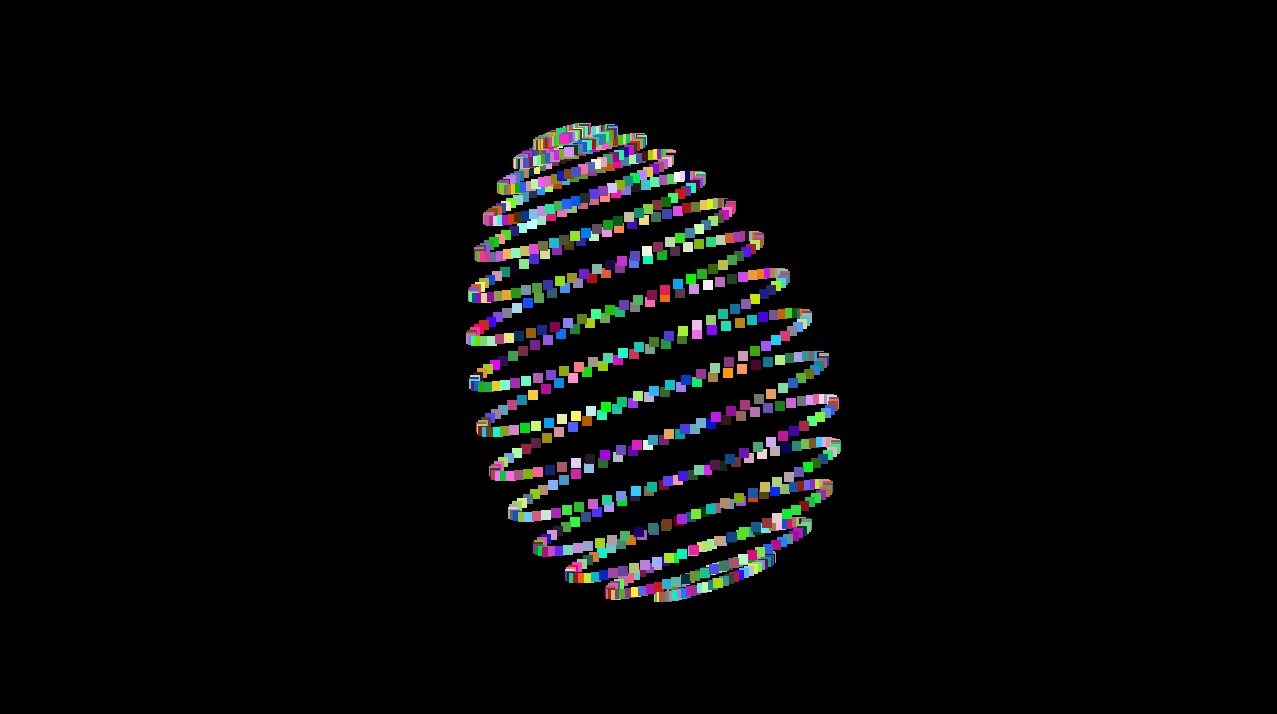
\includegraphics[width=\linewidth, trim={8cm 0 8cm 0},clip]{img/egg_1.png}
        \caption{Model jajka zbudowany z~punktów.}
    \end{minipage}
    \hspace{.05\linewidth}
    \begin{minipage}[t]{0.45\linewidth}
        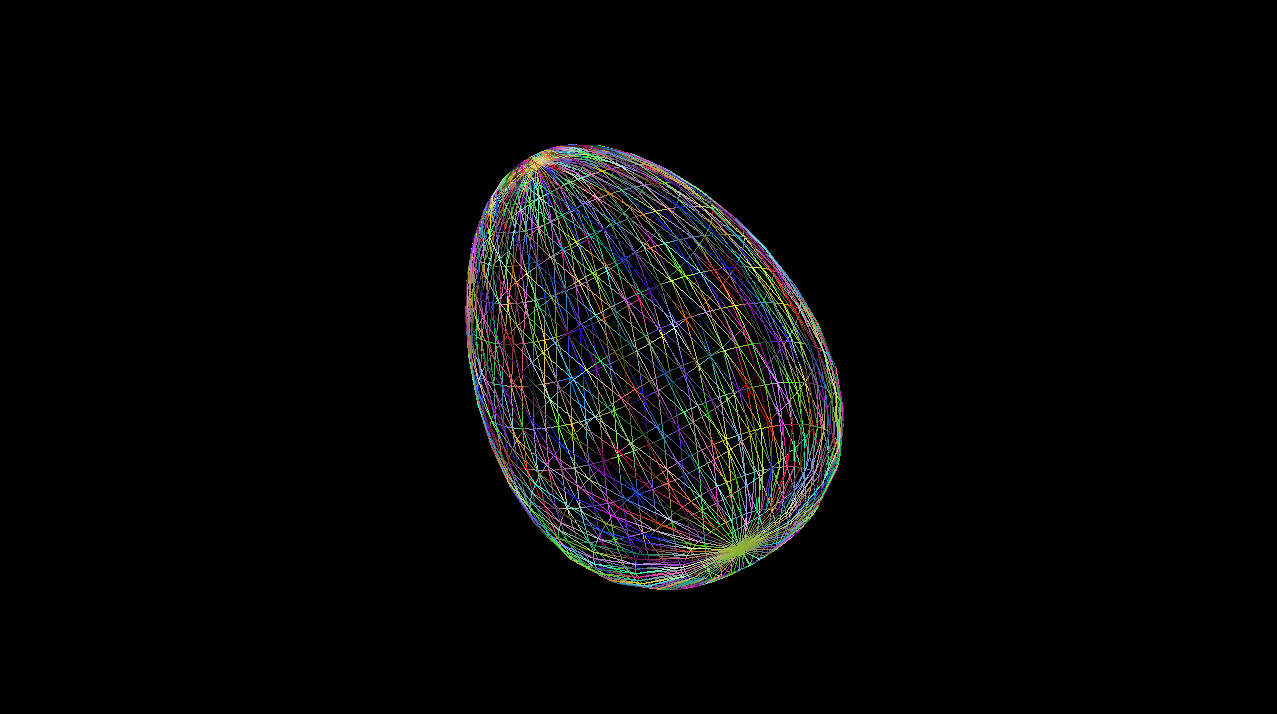
\includegraphics[width=\linewidth, trim={8cm 0 8cm 0},clip]{egg_2}
        \caption{Model jajka zbudowany z~siatki.}
    \end{minipage}
\end{figure}
\begin{figure}[h]
    \centering
    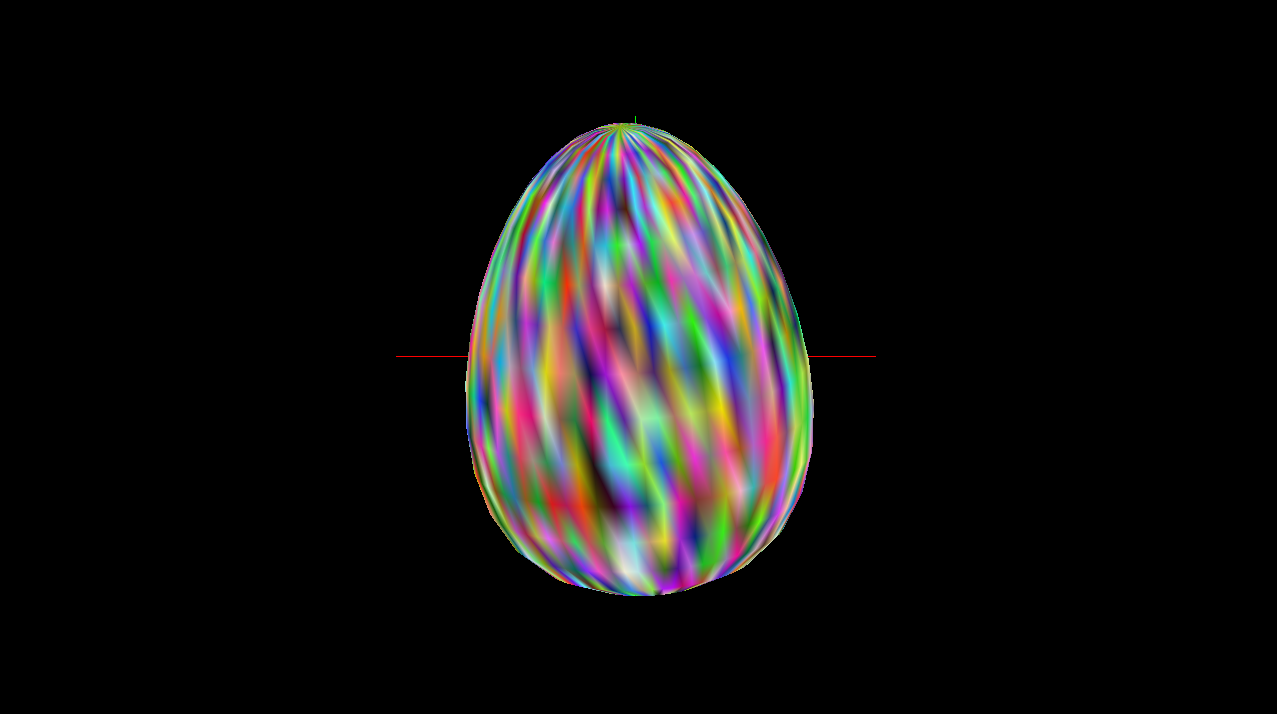
\includegraphics[width=0.45\linewidth, trim={8cm 0 8cm 0},clip]{img/egg_3.png}
    \caption{Model jajka zbudowany z~trójkątów.}
\end{figure}
\newpage
W przypadku rysowania za pomocą siatki wymagane było ujednolicenie losowo generowanych kolorów dla punktów, które w procesie ich generowania się na siebie nakładają. Ma to miejsce na czubkach oraz, w przypadku generowania dla całego zakresu $<0;1>$, dla jednego z \textit{południków} jajka.

\subsection{Animacja obrotu}
Zmiana kąta obrotu modelu odbywa się w metodzie \lstinline{IView::timer()} widoku, która wywoływana jest 60 razy na sekundę korzystając z funkcji \lstinline{void glutTimerFunc(unsigned int time, void (*callback)(int), int value)}. Zapewnia to większą kontrolę nad animacją i jej prędkością niż podanie wskaźnika do funkcji \lstinline{void glutIdleFunc(void (*callback)())}.
Metoda widoku inkrementuje zmienną definiującą kąt obrotu modelu dla rysowanej klatki. W listingu \ref{lst:anim}, podczas rysowania, przeprowadzony jest proces transformacji modelu. Najpierw resetowana jest macierz transformacji, potem dokonywany jest obrót o wartość ze zmiennej widoku wokół wszystkich osi. Translacja w osi $Y$ ustawia model \textit{mniej więcej} po środku ekranu.
\begin{lstlisting}[language=C++, caption=Ustawianie zmiennej kątu obrotu i przerysowanie klatki.]
void DotEggView::timer()
{
    eggRotation += 1;
    if (eggRotation >= 360)
        eggRotation = 0;
    glutPostRedisplay();
}
\end{lstlisting}

\newpage
\section{Interakcja z użytkownikiem}
W celu poszerzenia możliwości obsługi akcji użytkownika o zdarzenia myszy do interfejsu \lstinline{IView} opisanego na listingu \ref{lst:iView} dodano metody z listingu \ref{lst:intMethods}.

\begin{lstlisting}[language=C++, caption=Metody interfejsu IView do obsługi zdarzeń myszy., label={lst:intMethods}]
void onMouse(int btn, int state, int x, int y);
void onMotion(GLsizei x, GLsizei y) = 0;
\end{lstlisting}
W ogólnym przypadku metoda \lstinline{onMouse} zapisywała stan, klawisz przycisku myszy i jej pozycję, a metoda \lstinline{onMotion} odpowiadała za wykonywanie akcji odpowiedzialnej za ruch myszy.
\subsection{Perspektywa}
Za wyświetlenie perspektywiczne odpowiada metoda \lstinline{gluPerspective}, która zastąpiła metodę \lstinline{gluOrtho} odpowiedzialną za wyświetlanie ortograficzne w metodzie \lstinline{changeSize}. Widok obserwatora definiuje metoda \lstinline{gluLookAt}, do której poprzez parametry podane zostają pozycje kamery, celu i jej kierunku obrotu. W metodzie \lstinline{render} widoku \lstinline{TeapotView} dodane zostało wywołanie metody \lstinline{gluLookAt}, które argumenty czerpie ze zmiennych klasy widoku, co daje możliwość dowolnego sterowania pozycją obserwatora.
\begin{lstlisting}[language=C++, caption=Definicja i wywołanie metody \lstinline{gluLookAt}., label={lst:intGluLookAt}]
void gluLookAt(
    GLdouble eyeX, GLdouble eyeY, GLdouble eyeZ,
    GLdouble centerX, GLdouble centerY, GLdouble centerZ,
    GLdouble upX, GLdouble upY, GLdouble upZ
);
//---
gluLookAt(
    eye.x + center.x,eye.y + center.y, eye.z + center.z,
    center.x, center.y, center.z,
    0.0, 0.0, 1.0
);
\end{lstlisting}
\subsection{Transformacje widoku}
Transformacje widoku podzielono na trzy tryby, które obsługiwała metoda \lstinline{onMotion} w zależności od przyciśniętego klawisza.
\subsubsection{Obrót i skalowanie modelu}
Rysowany model imbryczka po naciśnięciu lewego przycisku myszy i jej przeciągnięciu jest obracany w osi Z i X oraz skalowany w przypadku naciśniętego prawego przycisku myszy. Użyto w tym celu parametryzowane transformacje \lstinline{glTranslate} i \lstinline{glRotate}. Aktualny kąty obrotu i skala są zapisywane w zmiennych klasy widoku i aktualizowana o ostatnią różnicę pozycji myszy.
\subsubsection{Obrót i zmiana pozycji kamery}
Pozycja kamery zapisywana jest jako zmienne określające środek sfery w położeniu $C$, o promieniu $R$, jej azymut $\Theta$ i kąt elewacji $\Phi$. Pozycja kamery w układzie współrzędnych wyliczana jest ze wzorów \ref{eq:1}.
\begin{subequations}
    \label{eq:1}
    \begin{align}  
        x(\Theta, \Phi) &= R \cdot cos(\Theta) \cdot cos(\Phi) + C_x\\
        y(\Theta, \Phi) &= R \cdot sin(\Theta) \cdot cos(\Phi) + C_y\\
        z(\Theta, \Phi) &= R \cdot sin(\Phi) + C_z
    \end{align}  
\end{subequations}
Aplikacja pozwala na manipulowanie kątami, promieniem, przemieszczeniem oraz odległością kamery od środka sfery.
\subsubsection{Obrót i zmiana pozycji świateł}
Światło reprezentowane jest jako klasa \lstinline{Light}. Światła, podobnie jak kamera, rozmieszczone są na powierzchni sfery ze środkiem w centrum układu współrzędnych. W trybie manipulacji źródłem światła można zmienić położenie jednego z dwóch świateł.
\clearpage
\section{Oświetlenie}
W celu odpowiedniego oddziaływania źródeł światła z powierzchnią modeli zdefiniowano dla nich materiał reprezentowany przez klasę \lstinline{Material}. Zawiera ona parametry \lstinline{ambient}, \lstinline{diffuse}, \lstinline{specular} i \lstinline{shininess}, definiujące kolejno współczynniki dla światła otoczenia, rozproszonego, odbitego oraz połysk powierzchni. Materiał używany jest poprzez wywołanie metody \lstinline{apply} pokazaną na listingu \ref{lst:mt:apply}.

\begin{lstlisting}[language=C++, caption=Metoda \lstinline{apply} klasy materiału., label={lst:mt:apply}]
void Material::apply()
{
  glMaterialfv(GL_FRONT, GL_SPECULAR, specular);
  glMaterialfv(GL_FRONT, GL_AMBIENT, ambient);
  glMaterialfv(GL_FRONT, GL_DIFFUSE, diffuse);
  glMaterialf(GL_FRONT, GL_SHININESS, shininess);
}
\end{lstlisting}


\begin{lstlisting}[language=C++, caption=Metody inicjujące światło na scenie., label={lst:light:init}]
void Light::calcPosition()
{
    position[0] = rDistance * cos(azimuth) * cos(elevation);
    position[1] = rDistance * sin(azimuth) * cos(elevation);
    position[2] = rDistance * sin(elevation);
    glLightfv(n, GL_POSITION, position);
}
void Light::calcColor()
{
    ambient[0] = color.r / 255. * 0.1;
    ...
    specular[2] = color.b / 255.;
    glLightfv(n, GL_AMBIENT, ambient);
    glLightfv(n, GL_DIFFUSE, diffuse);
    glLightfv(n, GL_SPECULAR, specular);
}


void Light::init(int n)
{
  this->n = n;
  calcColor(); calcPosition();
  glLightf(n, GL_CONSTANT_ATTENUATION, constant);
  glLightf(n, GL_LINEAR_ATTENUATION, linear);
  glLightf(n, GL_QUADRATIC_ATTENUATION, quadratic);
  glEnable(n);
}
\end{lstlisting}


Klasę \lstinline{Light} opisuje siedem parametrów: pozycja światła, współczynniki świecenia źródła światła otoczenia, światła powodującego odbicie dyfuzyjne i odbicie kierunkowe. Składają się na nie jeszcze składowa stała, liniowa i kwadratowa opisujące zmiany oświetlenia w zależności od odległości od jego źródła. Listing \ref{lst:light:init} przedstawia metody obliczające pozycję światła na powierzchni sfery, kolor dla wszystkich składowych oraz metody inicjujące te parametry na scenie.

\subsection{Oświetlenie imbryczka}
Na scenie został umieszczony imbryczek razem z dwoma źródłami światła. Ponieważ domyślnie nie są one reprezentowane przez żaden widzialny obiekt, ich pozycja została pokazana za pomocą sfer.
\begin{figure}[h]
    \centering
    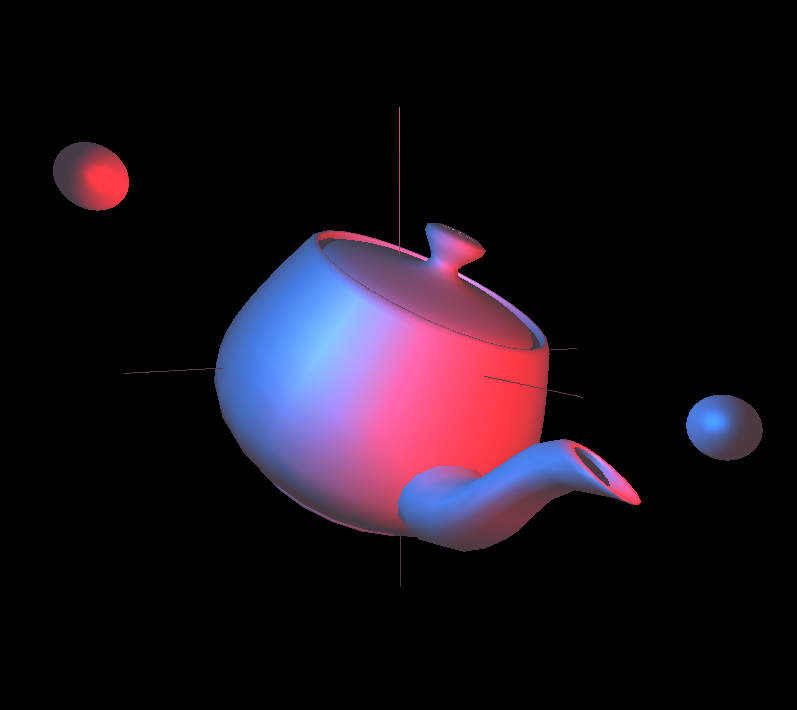
\includegraphics[width=0.55\linewidth, trim={0cm 3cm 0cm 3cm},clip]{img/teapot_1.png}
    \caption{Widok imbryczka z zastosowaną zmianą obrotu i skali modelu, zmianą położenia kamery, oświetlonego dwoma źródłami światła.}
\end{figure}
\begin{figure}[H]
    \centering
    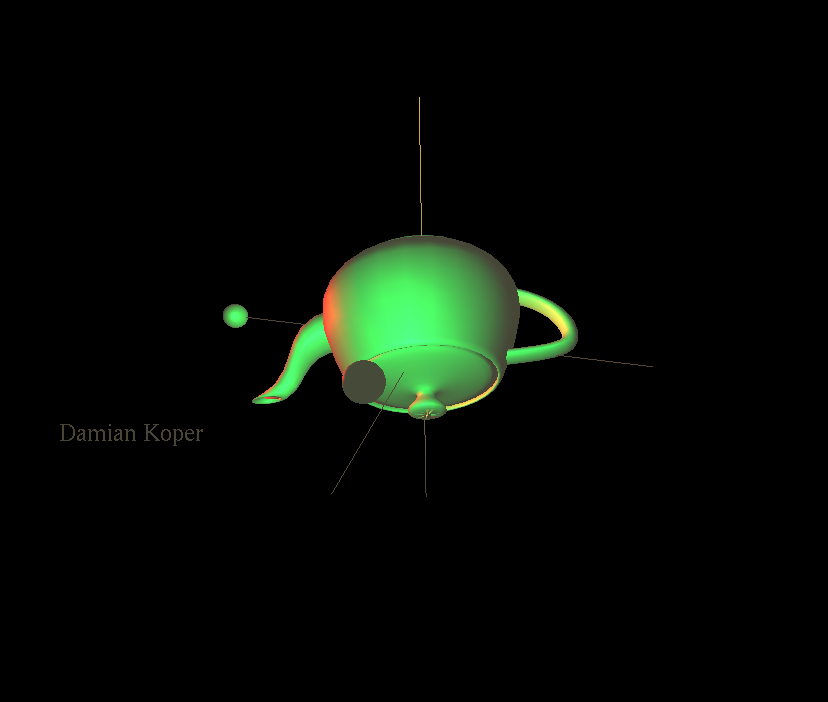
\includegraphics[width=0.8\linewidth, trim={0cm 6cm 0cm 2cm},clip]{img/teapot_2.png}
    \caption{Imbryczek w innej pozycji, widziany z innego punktu. Barwa światła znajdującego się bliżej kamery została zmieniona na zieloną.}
\end{figure}
\subsection{Oświetlenie jajka}
Wokół obracającego się modelu jajka zostały umieszczone dwa orbitujące pod różnym kątem i z różną prędkością źródła światła.
\begin{figure}[H]
    \centering
    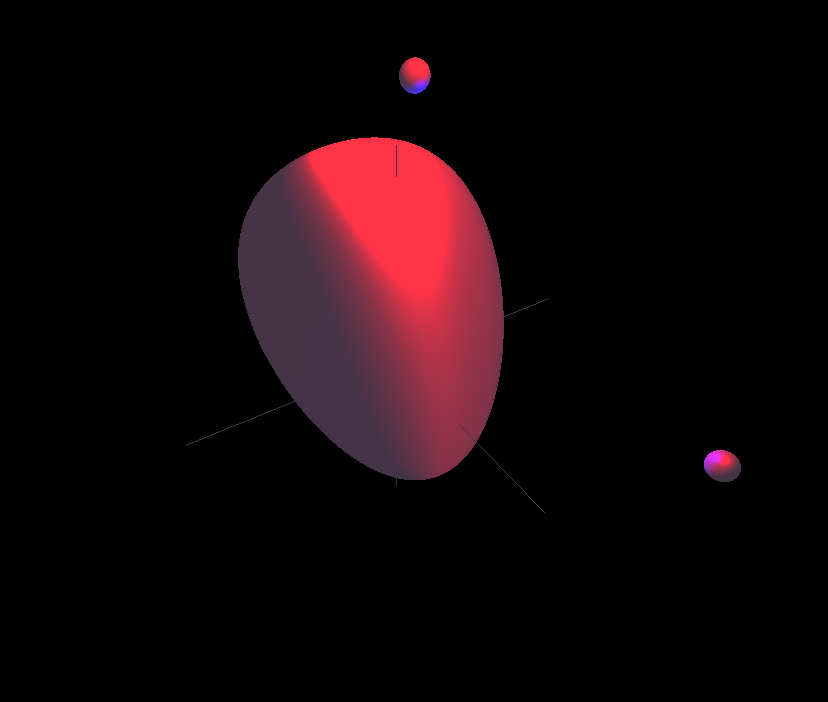
\includegraphics[width=0.8\linewidth, trim={0cm 6cm 0cm 0.5cm},clip]{img/egg_4.png}
    \caption{Oświetlony model jajka.}
\end{figure}
\newpage
\section{Teksturowanie}
Teksturowanie polega na nałożeniu na powierzchnię obiektu mapy bitowej. Mapa ta, by być właściwie nałożona na obiekt, musi być odpowiednio na nim odwzorowana. OpenGL pozwana określić odwzorowanie punktu trójkąta na punkt tekstury. Tekstura ładowana jest w postaci kwadratowej mapy bitowej o wielkości będącej potęgą liczby 2. W programie zastosowano tekstury z rastrowych plików graficznych w formacie \textit{TARGA} (.tga). 
Korzystanie z tekstur wymagało skonfigurowani odpowiednich parametrów oraz wywołania metody \lstinline{glEnable} z parametrem w odpowiednim widoku (listing \ref{lst:texturee}). Zastosowano opcję \textit{Cull Face}, która odpowiada za teksturowanie tylko jednej strony powierzchni, co redukuje obliczenia. W przypadku rysowania trójkątów, stronę powierzchni określa kolejność rysowania wierzchołków.

\begin{lstlisting}[language=C++, caption=Konfiguracja ustawień teksturowania., label={lst:texturee}]
glTexParameteri(GL_TEXTURE_2D, GL_TEXTURE_MAG_FILTER, GL_LINEAR);
glTexEnvi(GL_TEXTURE_ENV, GL_TEXTURE_ENV_MODE, GL_MODULATE);
...
glEnable(GL_TEXTURE_2D);
glEnable(GL_CULL_FACE);
\end{lstlisting}

\subsection{Klasa tekstury}
W celu zarządzania teksturami utworzona została klasa \lstinline{Texture}, która odpowiedzialna jest za wczytywanie, przetrzymywanie danych i wkładanie tekstury do bufora biblioteki OpenGL. Klasa ta przechowuje tablicę bajtów z danymi tekstury, jej wysokość i szerokość oraz format danych.
Przed narysowaniem danego modelu tekstura jest wkładana do bufora, za co odpowiedzialna jest metoda \lstinline{apply} pokazana na listingu \ref{lst:texture-apply}.
\clearpage
\begin{lstlisting}[language=C++, caption=Definicja klasy \lstinline{Texture}., label={lst:texture}]
class Texture
{
public:
    Texture(std::string filename);
    ~Texture();
    void apply();
private:
    GLbyte *pBytes;
    GLint width = 0;
    GLint height = 0;
    GLint components = GL_RGB8;
    GLenum format = GL_BGR_EXT;
};
\end{lstlisting}


\begin{lstlisting}[language=C++, caption=Metoda \lstinline{apply} klasy \lstinline{Texture}., label={lst:texture-apply}]
void Texture::apply()
{
    glTexImage2D(GL_TEXTURE_2D, 0, components, width, height, 0, format, GL_UNSIGNED_BYTE, pBytes);
}
\end{lstlisting}

\subsection{Klasa Point i model czworościanu}
By dodać możliwości teksturowania do obecnych modeli, modyfikacji uległa klasa \lstinline{Point}, do której zostały dodane współrzędne \textit{tx} i \textit{ty} określające odwzorowanie punktu w układzie współrzędnych tekstury. Wartości tych parametrów są liczbami z przedziału $<0;1>$. Punkt ten przekazywany jest do biblioteki OpenGL w metodzie rysującej \lstinline{drawWithColor}. Wywołanie odpowiedniej metody widoczne jest w linijce 5 listingu \ref{lst:point-dwc}.
\begin{lstlisting}[language=C++, caption=Konstruktor klasy \lstinline{Point}., label={lst:point-construct}]
Point(float x, float y, float z, GLubyte r, GLubyte g, GLubyte b, float tx = 0, float ty = 0)
        : color({r, g, b}), x(x), y(y), z(z), tx(tx), ty(ty){};

\end{lstlisting}
\begin{lstlisting}[language=C++, caption=Metoda \lstinline{drawWithColor} klasy \lstinline{Point}., label={lst:point-dwc}]
void Point::drawWithColor()
{
    color.apply();
    glNormal3f(nx, ny, nz);
    glTexCoord2f(tx, ty);
    glVertex3f(x, y, z);
}
\end{lstlisting}

Z tak zmodyfikowaną klasą \lstinline{Point} można było zdefiniować model \lstinline{TexModel}, którego konstruktor klasy tworzył punkty w odpowiedniej kolejności (listing \ref{lst:texmodel-con}), a metoda \lstinline{renderTriangles} rysowała je na ekranie (listing \ref{lst:texmodel-render}). 
\begin{lstlisting}[language=C++, caption=Konstruktor klasy \lstinline{TexModel}., label={lst:texmodel-con}]
TexModel::TexModel()
{
    points.push_back(std::vector<Point>({
        Point(1., 1., 0., 255, 255, 255, 1, 0),
        Point(5., 1., 0., 255, 255, 255, 0, 0),
        Point(3., 5., 0., 255, 255, 255, 0.5, 1)}));
    points.push_back(std::vector<Point>({
        Point(1., 1., 0., 255, 255, 255, 1, 0),
        Point(3., 2.5, 4., 255, 255, 255, 0.5, 1),
        Point(5., 1., 0., 255, 255, 255, 0, 0)}));
    points.push_back(std::vector<Point>({
        Point(3., 5., 0., 255, 255, 255, 1, 0),
        Point(5., 1., 0., 255, 255, 255, 0, 0),
        Point(3., 2.5, 4, 255, 255, 255, 0.5, 1)}));
    points.push_back(std::vector<Point>({
        Point(3., 2.5, 4, 255, 255, 255, 0.5, 1),
        Point(1., 1., 0., 255, 255, 255, 1, 0),
        Point(3., 5., 0., 255, 255, 255, 0, 0)}));
}
\end{lstlisting}
\clearpage
\begin{lstlisting}[language=C++, caption=Metoda \lstinline{renderTriangles} klasy \lstinline{TexModel}., label={lst:texmodel-render}]
void TexModel::renderTriangles()
{
    glBegin(GL_TRIANGLES);
    for (auto &&triangle : points)
    {
        for (auto &&point : triangle)
        {
            point.drawWithColor();
        }
    }
    glEnd();
}
\end{lstlisting}

\subsection{Wyświetlanie czworościanu i modelu jajka z teksturą}

W celu prezentacji wyświetlania modeli z teksturą utworzony został widok \lstinline{TexModelView}, gdzie w metodzie \lstinline{render} wyświetlane są dwa obracające się czworościany, na które zostały nałożony tekstury. Zostały one utworzone jako obiekty przechowywane w zmiennych klasy widoku.
\begin{lstlisting}[language=C++, caption=Zmienne klasy \lstinline{TexModelView} odpowiedzialne za model i tekstury., label={lst:texmodelview-hpp}]
TexModel texModel;
Texture texture1 = Texture("src/textures/paput.tga");
Texture texture2 = Texture("src/textures/D5_t.tga");
\end{lstlisting}

\begin{lstlisting}[language=C++, caption=Metoda \lstinline{render} klasy \lstinline{TexModelView}., label={lst:texmodelview-render}]
void TexModelView::render()
{
    glLoadIdentity();
    gluLookAt(5.0, 5.0, 10.0, 0.0, 0.0, 0.0, 0.0, 0.0, 1.0);
    DrawingUtils::axis();
    glPushMatrix();
    glRotated(eggRotation, 0, 0, 1);
    glPointSize(10.);
    texture1.apply();
    texModel.renderTriangles();
    glPopMatrix();
    glRotated(eggRotation+180, 0, 0, 1);
    glScaled(0.5,0.5,0.5);
    texture2.apply();
    texModel.renderTriangles();
}
\end{lstlisting}

\begin{figure}[H]
    \centering
    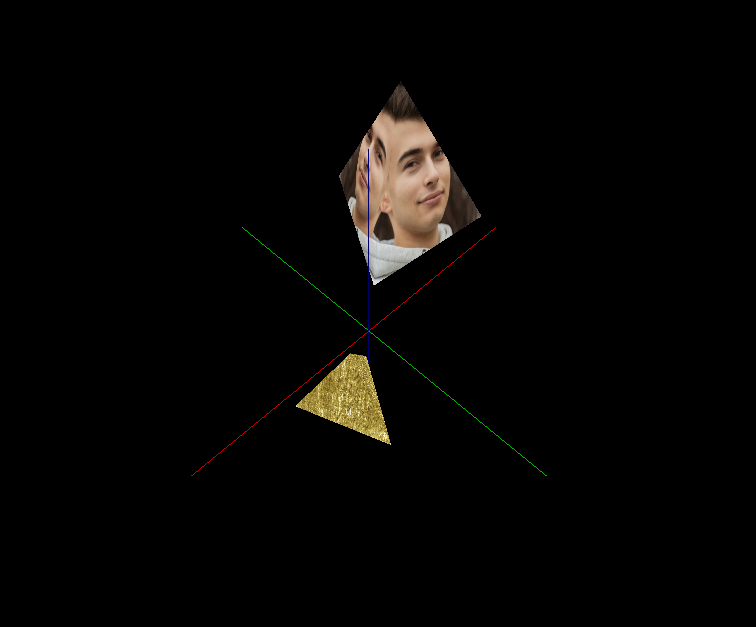
\includegraphics[width=0.8\linewidth, trim={0cm 4cm 0cm 2cm},clip]{img/tex_1.png}
    \caption{Obracające się dwa czworościany z nałożoną teksturą.}
\end{figure}


Dla modelu jajka punkty odwzorowania tekstury zostały przypisane zgodnie z naniesieniem ich na dziedzinę parametryczną równania opisującego model. Wykorzystano stworzony już wcześniej widok, w którym wyświetlane było jajko z przemieszczającymi się źródłami światła.

\begin{figure}[H]
    \centering
    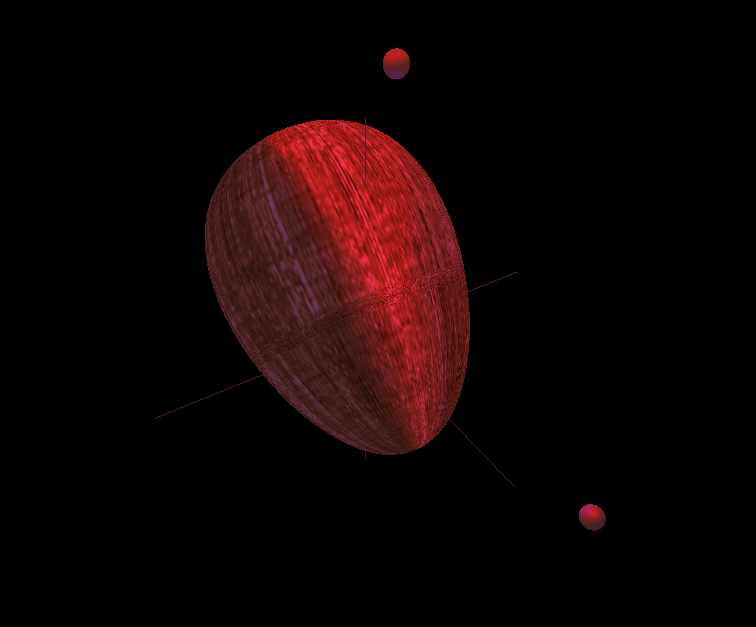
\includegraphics[width=0.8\linewidth, trim={0cm 2cm 0cm 1cm},clip]{img/tex_2.png}
    \caption{Obracający się model jajka z nałożoną teksturą i źródłami światła.}
\end{figure}


\end{document}